\documentclass[11pt,a4paper]{article}

\usepackage[a4paper,margin=1in]{geometry}
\usepackage{titlesec}
\usepackage{enumitem}
\usepackage{parskip}
\usepackage{tabularx}
\usepackage{fontspec}
\usepackage{graphicx}

% ใช้ฟอนต์คล้าย Google Docs
%language setting
\usepackage{fontspec}
\setmainfont{Roboto}

% ปรับหัวข้อ section
\titleformat{\section}
{\large\bfseries}
{}{0em}{}[\titlerule]

\begin{document}
\pagenumbering{gobble}
%====================
% HEADER
%====================

\begin{minipage}{0.75\textwidth}
{\LARGE \textbf{Chonlathit Phuncam}}\\
{\LARGE \textbf{Aomsin}}\\
Ratchaburi, Thailand \\
090-6324894 | phuncam.c@gmail.com \\
https://www.linkedin.com/in/chonlathitp \\
https://linktr.ee/kyo.skykim\\
\end{minipage}
\hfill
\begin{minipage}{0.2\textwidth}
\begin{flushright}
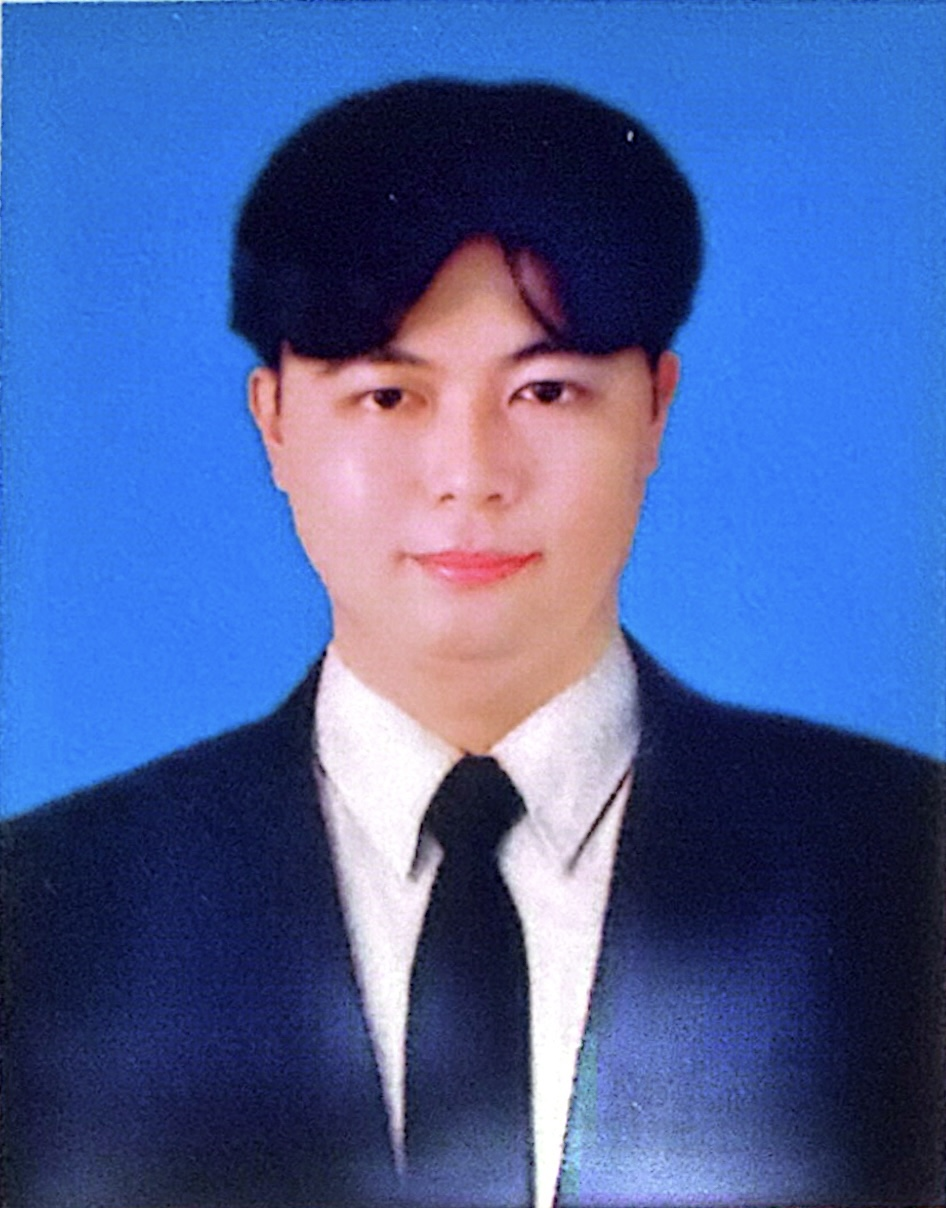
\includegraphics[width=4cm]{profile.jpg}
\end{flushright}
\end{minipage}
%====================
% PROFILE
%====================

\section*{PROFILE}
\textbf{Concepts: Data Engineer, Data Visualization, Data Modeling, Financial Mathematics} \\
Bachelor of Science in Mathematics with coursework in Mathematical Analysis, Appiled Mathematics and Elementary Statistics. Currently attending a Data Engineering through intensive bootcamp training.

Adept at logical problem-solving and applying mathematical principles to analyze complex datasets and support data-driven decision-making.

%====================
% EDUCATION
%====================

\section*{EDUCATION}

\begin{tabularx}{\textwidth}{p{3cm} X r}
2026 -- Present &
\textbf{Data Engineering Bootcamp (In Progress)} & \small{Thailand} \\
& Databricks for Data Engineers Bootcamp 2 & \\

2017 -- 2022 &
\textbf{Bachelor of Science (Mathematics)} & \small{Nakhon Pathom, Thailand} \\
& Silpakorn University & \\

2012 -- 2017 &
\textbf{Benjamarachutit Ratchaburi School} & \small{Ratchaburi, Thailand} \\
\end{tabularx}

%====================
% EXPERIENCE
%====================

\section*{EXPERIENCES \& ACTIVITIES}

\begin{tabularx}{\textwidth}{l X r}
2023 -- Present & 
\textbf{Mathematics Tutor} & 
\small{Ratchaburi, Thailand} \\

& \begin{itemize}[leftmargin=*, nosep, after=\vspace{-\baselineskip}]
    \item \textbf{Analyzed student data} to identify learning gaps and optimize teaching strategies.
    \item \textbf{Simplified complex concepts} for clear and effective communication.
\end{itemize} & 
\end{tabularx}

\vspace{0.3cm}

\begin{tabularx}{\textwidth}{l X r}
2021 -- 2022 & 
\textbf{Staff of Academic Olympaid Camp (POSN2)} & 
\small{Silpakorn University} \\
&
\begin{itemize}
        \item \textbf{Collected and cleaned} student data from Excel (survey responses)
        \item \textbf{Built interactive dashboard} using Looker Studio
        \item \textbf{Analyzed} food allergies, medical conditions, and insurance data
        \item Supported planning and risk management using data insights
    \end{itemize}
\end{tabularx}

\begin{tabularx}{\textwidth}{l X r}
2020 -- 2022 &
\textbf{Student Council} &
\small{Faculty of Science} \\
&
\begin{itemize}
    \item Assisted in \textbf{planning and managing faculty events} with large student participation
    \item Promoted to vice leader in 2022
\end{itemize}
\end{tabularx}

\section*{Research Project}
\begin{tabularx}{\textwidth}{p{2.5cm} X >{\raggedleft\arraybackslash}p{4cm}}
\begin{tabular}[t]{@{}l@{}}2026 \\ \small{(In progress)}\end{tabular} & 
\small\textbf{Automated Ethereum Data Pipeline \& Anomaly Detection} & \small{Independent Study} \\
&
    \begin{itemize}
        \item \textbf{Developed an end-to-end ETL pipeline} use Python to extract Ethereum with robust error handling.
        \item \textbf{Processed and transformed data} use PySpark and Spark SQL on Databricks with explicit schema definitions.
        \item \textbf{Applied statistical methods} using SQL window functions to systematically detect price spikes and crashes.
        \item \textbf{Designed dashboard} to visualize for data-driven insights.
    \end{itemize}
\end{tabularx}

\begin{tabularx}{\textwidth}{p{2.5cm} X >{\raggedleft\arraybackslash}p{4cm}}
2022 &
\small\textbf{Injectivity and quasi-injectivity of products of some polynomials and Dedekind psi function} & 
\begin{tabular}[t]{@{}r@{}}\small{Undergraduate} \\ \small{Research Project}\end{tabular} \\
&
    \begin{itemize}
        \item \textbf{Applied MATLAB} to analyze numerical patterns and detect duplicate function outputs
        \item \textbf{Performed data} matching and validation using Excel
        \item \textbf{Documented findings and presented} analytical results in a structured format
    \end{itemize}
\end{tabularx}



%====================
% SKILLS
%====================

\section*{SKILLS}
\begin{itemize}
    \item \textbf{Data Engineering}: ETL/ELT Pipelines, Data Modeling (Star Schema), Delta Lake
    \item \textbf{Data Analysis}: Exploratory Data Analysis (EDA), Statistical Analysis, Data Cleaning
       \item \textbf{Data Visualization}: Looker Studio, Databricks, Excel
    \item \textbf{Programming}: Python (NumPy, Pandas, PySpark), R, MATLAB, SQL
    \item \textbf{Tools}: Databricks, Excel, PowerPoint, LaTeX, AI
\end{itemize}

%====================
% LANGUAGES
%====================

\section*{LANGUAGES}

\begin{tabular}{ll}
Thai & Native \\
English & Intermediate \\
Japanese & Beginning
\end{tabular}

\section*{CERTIFICATIONS}
\begin{enumerate}[leftmargin=*]
\item Data Science for Everyone -- Future Skills (2026)
\item Power BI Data Transformation (Power Query) -- Future Skills (2026)
\item AI with Data Visualization -- Future Skills (2025)
\item SQL for Data Analysis -- Future Skills (2025)
\item Push It with Data -- Chula MOOC (2025)
\end{enumerate}
\end{document}